%%%%%%%%%%%%%%%%%%%%%%%%%%%%%%%%%%%%%%%%%%%%%%%%%%%%%%%%%%%%%%%%
%%%%%%%%%%%%%%%%%%%%%%%%%%%%%%%%%%%%%%%%%%%%%%%%%%%%%%%%%%%%%%%%
%%%%
%%%% This text file is part of the source of 
%%%% `Introduction to High-Performance Scientific Computing'
%%%% by Victor Eijkhout, copyright 2012
%%%%
%%%% This book is distributed under a Creative Commons Attribution 3.0
%%%% Unported (CC BY 3.0) license and made possible by funding from
%%%% The Saylor Foundation \url{http://www.saylor.org}.
%%%%
%%%%
%%%%%%%%%%%%%%%%%%%%%%%%%%%%%%%%%%%%%%%%%%%%%%%%%%%%%%%%%%%%%%%%
%%%%%%%%%%%%%%%%%%%%%%%%%%%%%%%%%%%%%%%%%%%%%%%%%%%%%%%%%%%%%%%%

There are several informal ways of measuring just `how big' a computer
is. The most popular is the TOP500 list, maintained at
\url{http://www.top500.org/}, which records a computer's performance
on the \indextermbus{Linpack}{benchmark}. \indexterm{Linpack} is a
package for linear algebra operations, and no longer in use, since it
has been superseded by \indexterm{Lapack} for shared memory and
\indexterm{Scalapack} for distritubed memory computers. The benchmark
operation is the solution of a (square, nonsingular, dense) linear
system through LU factorization with partial pivoting, with subsequent
forward and backward solution.

The LU factorization operation is one that has great opportunity for
cache reuse, since it is based on the matrix-matrix multiplication
kernel discussed in section~\ref{sec:gemm}. It also has the property
that the amount of work outweighs the amount of communication:
$O(n^3)$ versus~$O(n^2)$.
As a result, the 
Linpack benchmark is likely to run at a substantial fraction of the
peak speed of the machine. Another way of phrasing this is to say that
the Linpack benchmark is a \indexterm{CPU-bound algorithm}.

Typical efficiency figures are between 60 and 90 percent. However, it
should be noted that many scientific codes do not feature the dense
linear solution kernel, so the performance on this benchmark is not
indicative of the performance on a typical code. Linear system
solution through iterative methods (section~\ref{sec:iterative}), for
instance, is much less efficient in a flops-per-second sense, being
dominated by the bandwidth between CPU and memory
(a~\indexterm{bandwidth bound algorithm}).

One implementation of the Linpack benchmark that is often used is
`High-Performance LINPACK'
(\url{http://www.netlib.org/benchmark/hpl/}), which has several
parameters such as blocksize that can be chosen to tune the performance.

\Level 2 {The top500 list as a recent history of supercomputing}

The top500 list offers a history of almost 20 years of
supercomputing. In this section we will take a brief look at
historical developments\footnote{The graphs contain John McCalpin's
  analysis of the top500 data.}. First of all,
figure~\ref{fig:top500-types} shows the evolution of architecture types
\begin{figure}[ht]
%  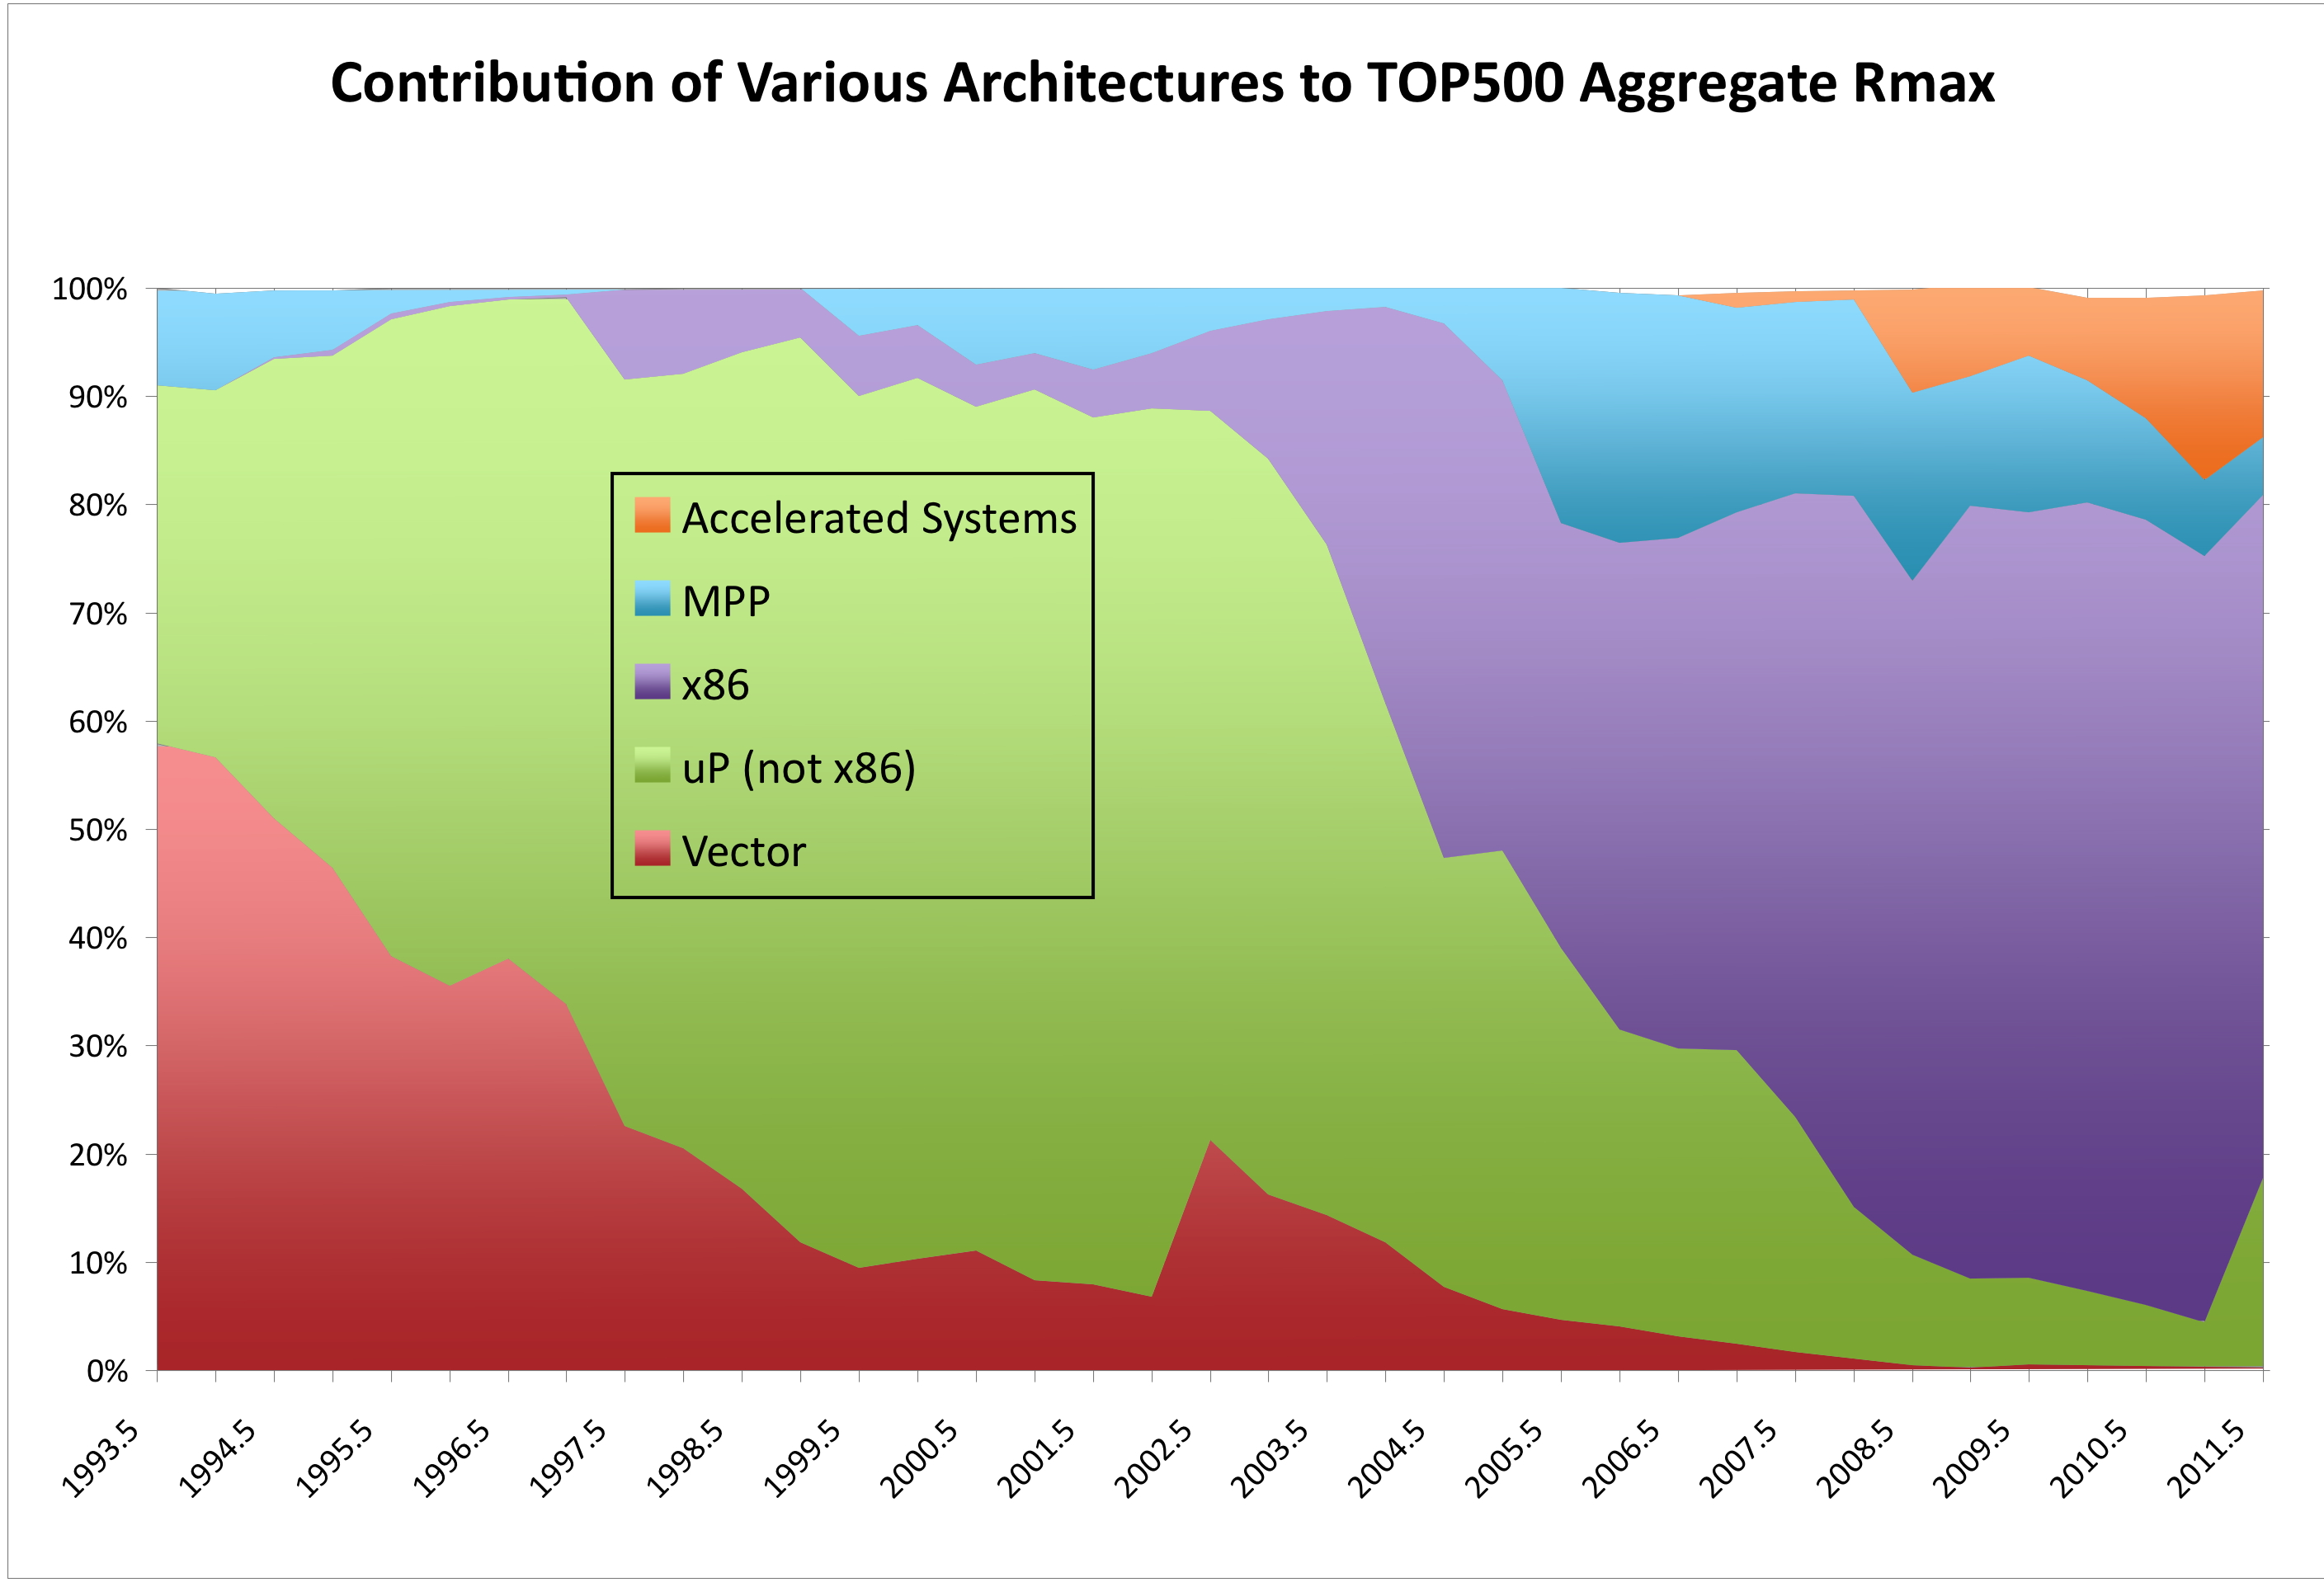
\includegraphics[scale=.6]{graphics-public/top500/types}
  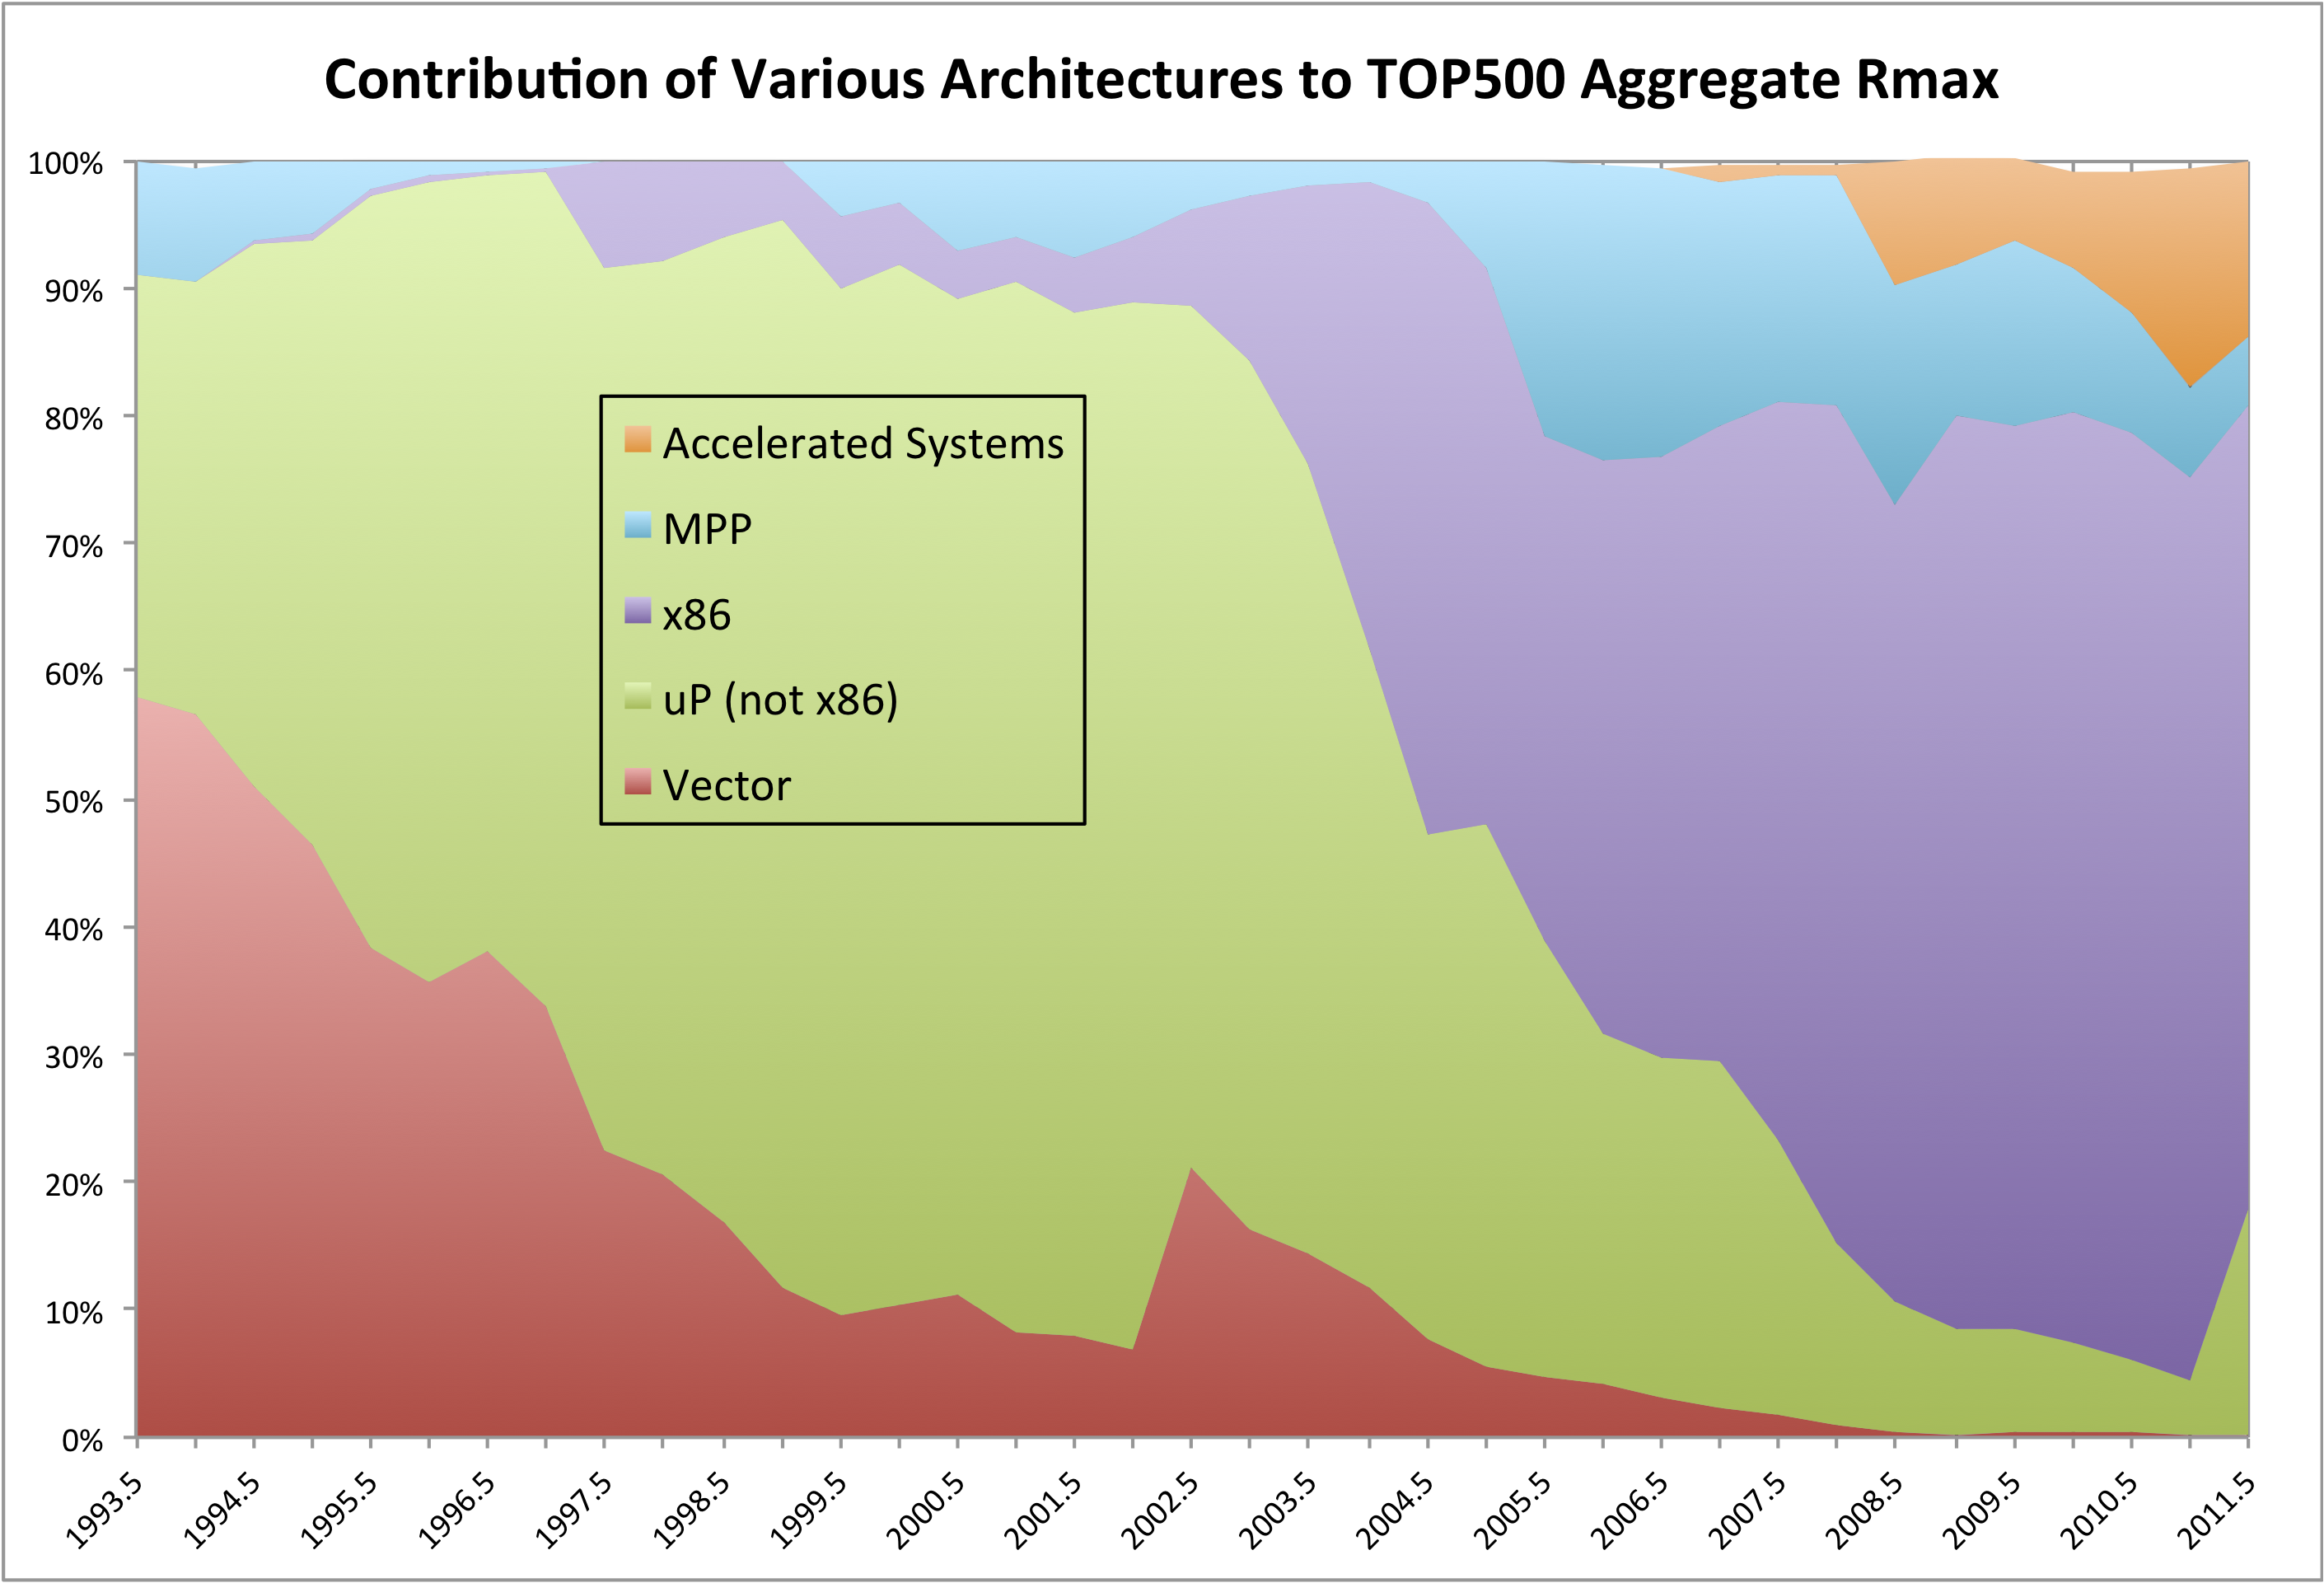
\includegraphics[scale=.6]{graphics-public/top500/ChartByArchitecture}
  \caption{Evolution of the architecture types on the top500 list}
  \label{fig:top500-types}
\end{figure}
by charting what portion of the aggregate peak performance of the
whole list si due to each type.
\begin{itemize}
\item Vector machines feature a relatively small number of very powerful vector
  pipeline processors (section~\ref{sec:vector}). This type of
  architecture has largely disappeared; the last major machine of this
  type was the Japanese \indexterm{Earth Simulator} which is seen as
  the spike in the graph around 2002, and which was at the top of the
  list for two years.
\item Micro-processor based architectures get their power from the
  large number of processors in one machine. The graph distinguishes
  between \indexterm{x86} (\indexterm{Intel} and \indexterm{AMD}
  processors with the exception of the \indextermbus{Intel}{Itanium})
  processors and others; see also the next graph.
\item A number of systems were designed as highly scalable
  architectures: these are denoted MPP for `massively parallel
  processor'. In the early part of the timeline this includes
  architectures such as the \indexterm{Connection Machine}, later it
  is almost exclusively the \indextermbus{IBM}{BlueGene}.
\item In recent years `accelerated systems' are the upcoming
  trend. Here, a processing unit such as a \indexac{GPU} is attached
  to the networked main processor.
\end{itemize}
Next, figure~\ref{fig:top500-processor} shows the dominance of the
\indexterm{x86} processor type relative to other micro-processors.
\begin{figure}[ht]
  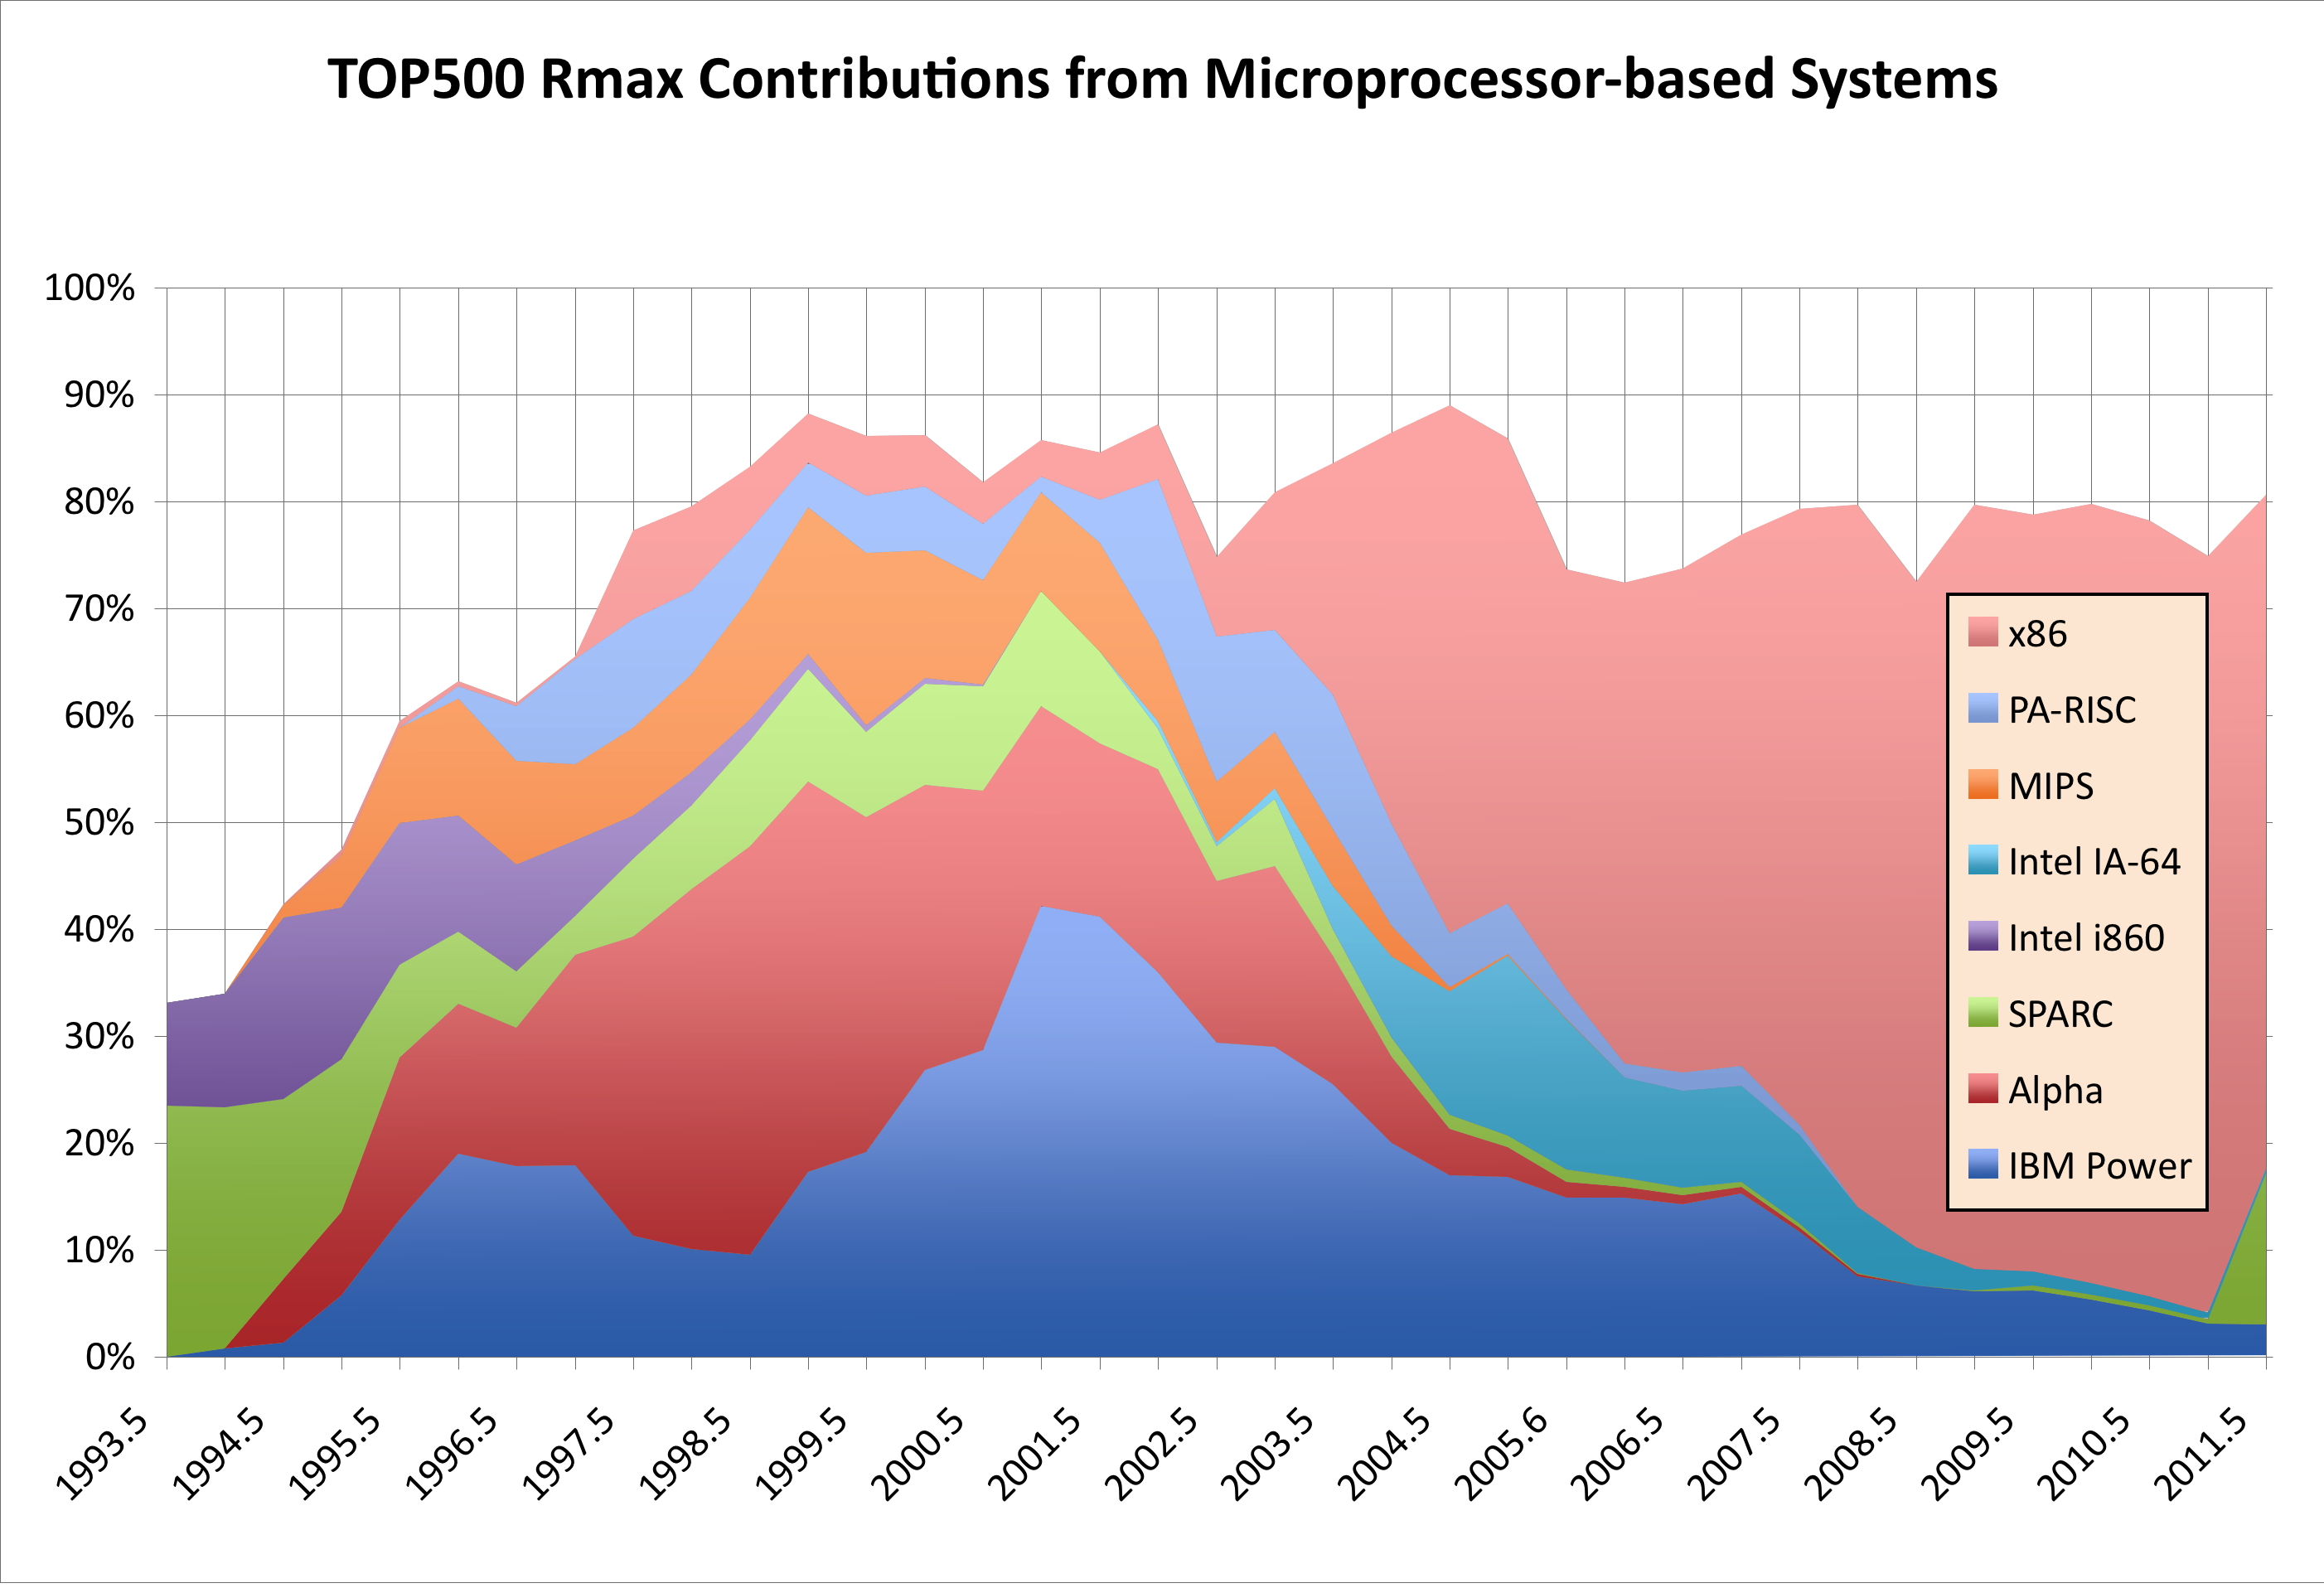
\includegraphics[scale=.6]{graphics-public/top500/processor}
  \caption{Evolution of the architecture types on the top500 list}
  \label{fig:top500-processor}
\end{figure}
(Since we classified the \indextermbus{IBM}{BlueGene} as an MPP, its
processors are not in the `Power' category here.)

Finally, figure~\ref{fig:top500-cores} shows the gradual increase in
core count. Here we can make the following observations:
\begin{figure}[ht]
  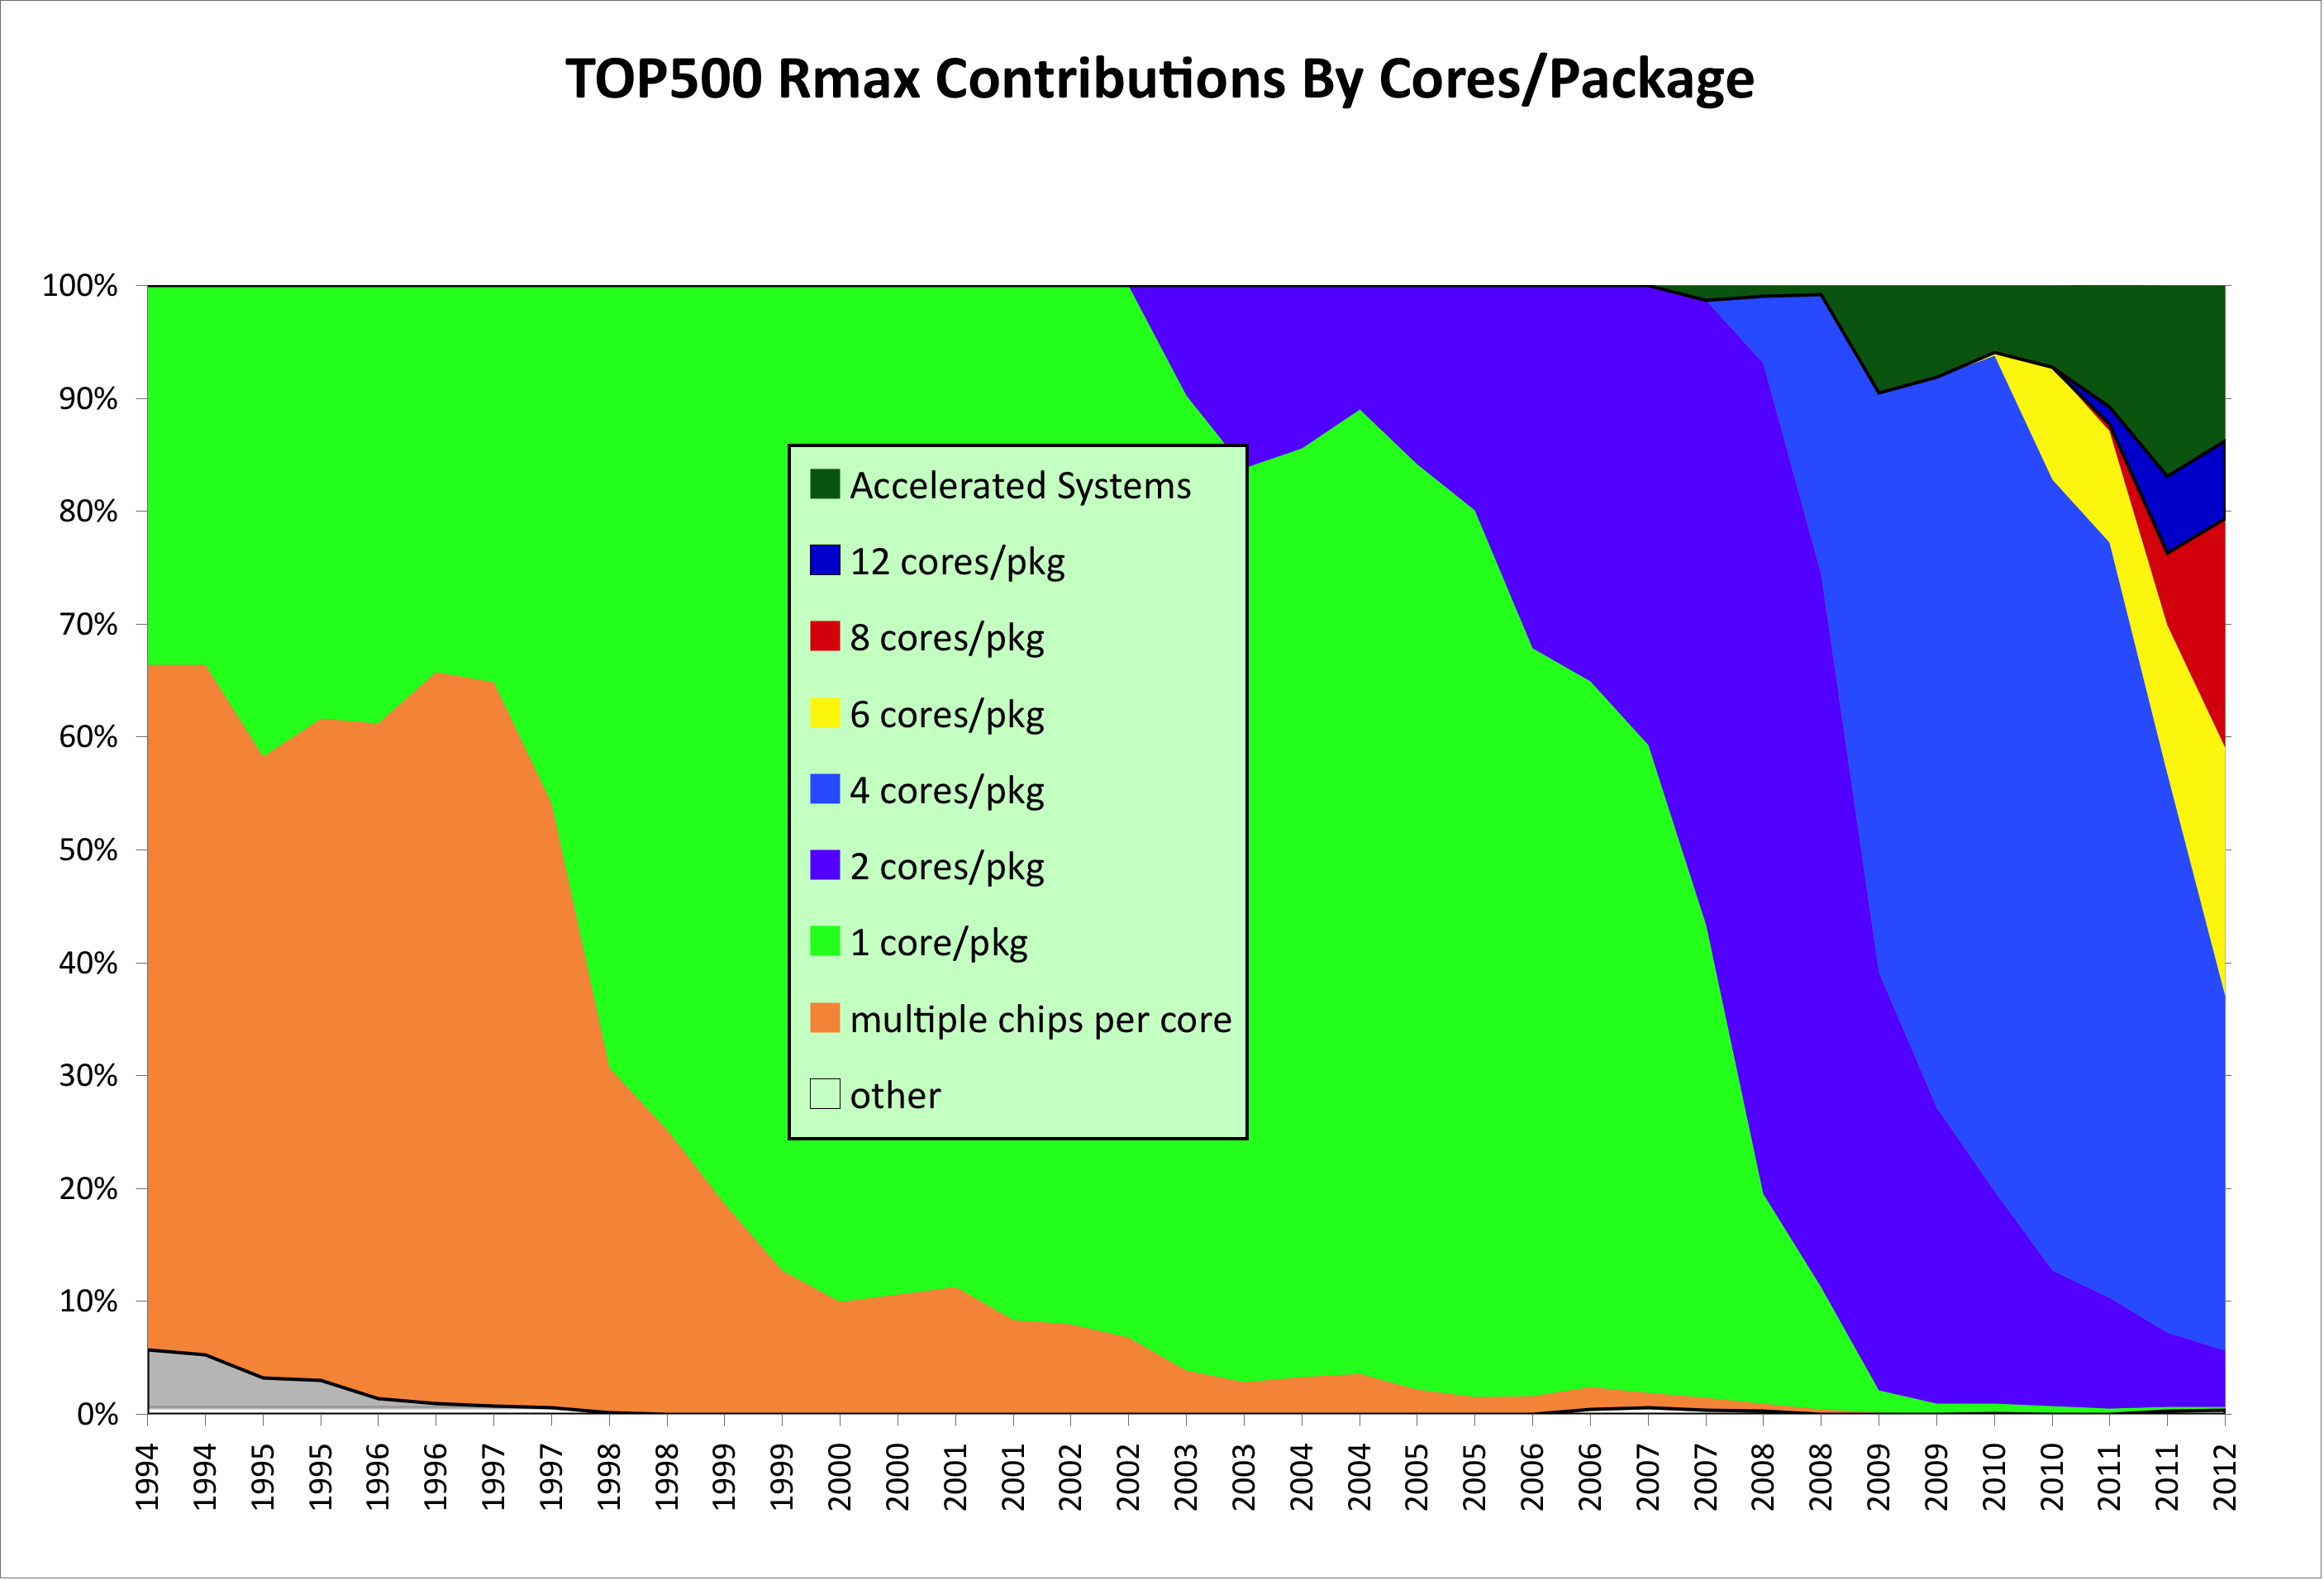
\includegraphics[scale=.6]{graphics-public/top500/cores}
  \caption{Evolution of the architecture types on the top500 list}
  \label{fig:top500-cores}
\end{figure}
\begin{itemize}
\item In the 1990s many processors consisted of more than one chip.
  In the rest of the graph, we count the number of cores per
  `package', that is, per \indexterm{socket}. In some cases a socket
  can actually contain two separate dies.
\item With the advent of multi-core processors, it is remarkable how
  close to vertical the section in the graph are. This means that new
  processor types are very quickly adopted, and the lower core counts
  equally quickly completely disappear.
\item For accelerated systems (mostly systems with \acp{GPU}) the
  concept of `core count' is harder to define; the graph merely shows
  the increasing importance of this type of architecture.
\end{itemize}
